\begin{anexosenv}

\partanexos

\chapter{Sistema Geral}
\begin{figure}[h]
	\centering
	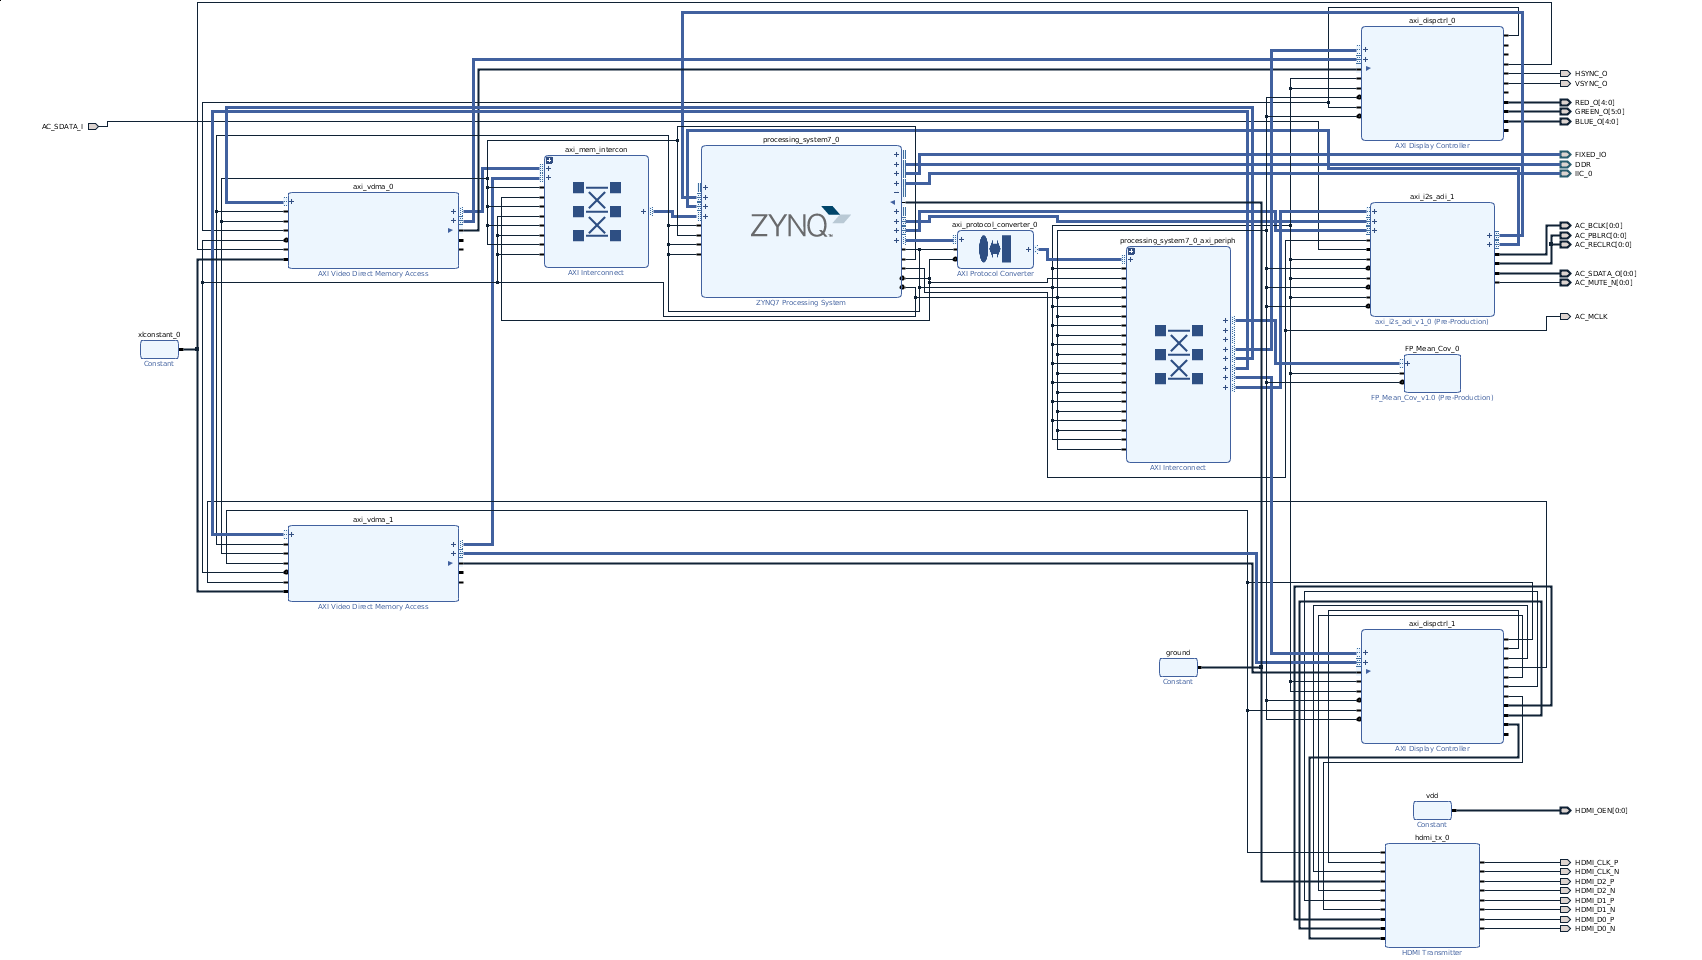
\includegraphics[keepaspectratio=true,scale=0.32, angle=90]{figuras/base-zybo.png}
	\caption{Sistema geral com IP}
	\label{sitemageral}
\end{figure}



\chapter{Tutorial para Instalação do Sistema Operacional Linux no Zybo}

 Este tutorial foi elaborado para ambiente Linux e baseia-se no tutorial disponibilizado por \cite{tutorialzybo}.
 
 \subsection{Geração do Arquivo u-boot.elf}
 \subsubsection{Requisitos Necessários}
\begin{itemize}
\item Vivavo 2014.1 WebPACK ou superior, disponivel em : \url{https://www.xilinx.com/support/download.html}
\item Acesso ao repositório no git para "u-boot-xlnx" disponível em : \url{https://github.com/Xilinx/u-boot-xlnx} 

\end{itemize} 
\subsubsection{Instruções}
Para começarmos precisamos baixar o reposítório do u-boot, para isso usamos o comando:
\begin{lstlisting}[language=bash]
$git clone https://github.com/Xilinx/u-boot-xlnx.git
\end{lstlisting}
Este comando faz o download do repositório u-boot-xlnx mantindo pela Xilinx, em seguida entramos no diretório:

\begin{lstlisting}[language=bash]
$cd u-boot-xlnx/
\end{lstlisting}
Dentro do diretório, é necessário carregar as ferramentas de compilação, vamos usar o comando:

\begin{lstlisting}[language=bash]
$source /opt/Xilinx/Vivado/2017.4/settings64.sh
\end{lstlisting}
Neste ponto iremos limpar todos os arquivos já compilados que podem estar no repositório, para isso usamos os seguintes comandos:
\begin{lstlisting}[language=bash]
$make mrproper
$make clean
\end{lstlisting}
Agora vamos adicionar as variáveis de ambiente para compilação e o arquivo de configuração para o kit Zybo com os comandos abaixo:
\begin{lstlisting}[language=bash]
$make CROSS_COMPILE=arm-linux-gnueabihf- zynq_zybo_config
\end{lstlisting}
o arquivo de configuração foi criado, para compilar usamos o comando:
\begin{lstlisting}[language=bash]
$make CROSS_COMPILE=arm-linux-gnueabihf-
\end{lstlisting}
Por fim vamos adicionar a extensão ".elf" ao arquivo "u-boot", usaremos o seguite comando:
\begin{lstlisting}[language=bash]
$mv u-boot u-boot.elf
\end{lstlisting}

Esta etapa foi concluida, vamos agora criar o aquivo BOOT.bin.


 
 

\subsection{Geração do Arquivo BOOT.bin}
Requisitos Necessários:
\begin{itemize}
\item Vivavo 2014.1 WebPACK ou superior, disponivel em : \url{https://www.xilinx.com/support/download.html}
\item ZYBO \textit{Base Sytem Design}  disponível em: \url{https://reference.digilentinc.com/_media/reference/programmable-logic/zybo/zybo_base_system.zip}
\item completar o passo anterior

\end{itemize}



\subsubsection{Instruções}
Para criarmos o arquivo BOOT.bin  primeiramente descompactamos o aquivo "zybo\_base\_sytem.zip", podemos usar o seguinte comando:

\begin{lstlisting}[language=bash]
$unzip zybo_base_system.zip
\end{lstlisting}

Após descompactar iremos até o diretório:

\begin{lstlisting}[language=bash]
$zybo_base_system/source/vivado/hw/zybo_bsd/
\end{lstlisting}

Com o software vivado iremos abrir o arquivo "zybo\_bsd.xpr".
No vivado executaremos a função: \textbf{Generate Bitstream}.
 
\textit{obs: Isse passo irá demorar alguns minutos.}

Agora exportaremos o ".bit" para a pasta de projeto, no Vivado siguimos os passos: \textbf{File > Export > Export Hardware} na janela que surgirá, marcaremos a opção \textbf{Include Bitstream}.
Ainda no Vivado façamos os passos: \textbf{File > Launch SDK}

\textit{obs: Todos os passos agora serão executados do software SDK}

No SDK vamos criar o aquivo fsbl.elf (first stage boot loader). Este é responsável por carregar o arquivo de configuração (bitstream) no sistema de processamento do Zybo. Para cria-lo vamos seguir os passos: \textbf{File > New > Aplication Project} no campo "Project Name" usaremos "fsbl" e clicamos em \textbf{Next}, agora escolheremos o tamplate \textbf{Zynq FSBL}, por fim clicamos em \textbf{Finish}.\\

Neste ponto estamos de posse dos arquivos \textbf{u-boot.elf, fsbl.elf e system\_wraper.bit}, estes são necessários para gerarmos o \textbf{BOOT.bin}.

Seguiremos então os passos: \textbf{Xilinx > Criate Boot Image}, na janela que surgirá escolhemos o diretório de saída de nossa preferência. No campo "Boot Image Partitions", iremos adicionar os seguintes aquivos em ordem; \textit{obs: A ordem dos aquivos é muito importante para esse processo.}
em \textbf{Add} adicionaremos o aquivo \textbf{fsbl.elf} que se encontra na pasta de projeto:
\begin{lstlisting}[language=bash]
zybo_bsd.sdk/fsbl/Debug/fsbl.elf
\end{lstlisting}
Posteriormente adicionaremos o aquivo \textbf{system\_wraper.bit} que se encontra no diretório:
\begin{lstlisting}[language=bash]
zybo_bsd.sdk/system\wrapper_bsd_plataform_hw_0/system_wrapper.bit
\end{lstlisting}
e por fim o arquivo \textbf{u-boot.elf}, que se encontra no diretório que clonamos do git:
\begin{lstlisting}[language=bash]
u-boot-xlnx/u-boot.elf
\end{lstlisting}
Com esses três arquivos adicionados clicamos em \textbf{Criate Image}. No diretório de saída que escolhemos estará o arquivo \textbf{BOOT.bin}.


\section{Compilando o Kernel Linux}
\subsection{Requisitos Necessários}
\begin{itemize}
\item Vivavo 2014.1 WebPACK ou superior, disponivel em : \url{https://www.xilinx.com/support/download.html}
\item ZYBO \textit{Base Sytem Design}  disponível em: \url{https://reference.digilentinc.com/_media/reference/programmable-logic/zybo/zybo_base_system.zip}
\end{itemize}

\subsubsection{Instruções}

Para começarmos precisamos baixar o reposítório do linux-xlnx, para isso usamos o comando:
\begin{lstlisting}[language=bash]
$git clone https://github.com/Xilinx/linux-xlnx.git
\end{lstlisting}
Este comando faz o download do repositório linux-xlnx mantindo pela Xilinx, em seguida entramos no diretório:

\begin{lstlisting}[language=bash]
$cd linux-xlnx/
\end{lstlisting}
Dentro do diretório, é necessário carregar as ferramentas de compilação, vamos usar o comando:

\begin{lstlisting}[language=bash]
$source /opt/Xilinx/Vivado/2017.4/settings64.sh
\end{lstlisting}
Neste ponto iremos limpar todos os arquivos já compilados que podem estar no repositório, para isso usamos os seguintes comandos:
\begin{lstlisting}[language=bash]
$make mrproper
$make clean
\end{lstlisting}
Agora vamos adicionar as variáveis de ambiente para compilação e o arquivo de configuração para o kit Zybo com os comandos abaixo:
\begin{lstlisting}[language=bash]
$make ARCH=arm CROSS_COMPILE=arm-linux-gnueabihf- xilinx_zynq_defconfig
\end{lstlisting}
o arquivo de configuração foi criado, para compilar o kernel usamos o comando:
\begin{lstlisting}[language=bash]
$make ARCH=arm CROSS_COMPILE=arm-linux-gnueabihf-
\end{lstlisting}
\textit{obs: Este comando pode demorar alguns minutos para terminar.}

















\end{anexosenv}

